\section{Conclusion}


\begin{frame}[noframenumbering]
	
\vfill
\centering

\vspace{-.5cm}\textbf{\Large Concluding}\vspace{-.5cm}

\vfill

\centering

\end{frame}



\begin{refframe}{Translating Back to Physics}

\centering

%\footnotesize Local Hamiltonian Problem}
\tikzset{venn circle/.style={circle,minimum width=2cm,fill=####1,opacity=0.4}}
\begin{tikzpicture}[
e/.style = {ellipse, fill=####1, draw=none,
            minimum height=.7cm, minimum width=.9cm, inner sep=0pt},
e/.default=black
]
\footnotesize


%\draw[help lines] (0,0) grid (4,3);


  \node [e = yellow!0!red!80!white,text width=2.8cm,align=center, minimum width=.8cm,  minimum height=3.6cm,text opacity=1,label={[anchor=north, inner sep=3pt,yshift=-.25cm]north:Precise\QMA = \PSPACE}] (PSPACE) at (.8,0.5) {};
	\node[right = of PSPACE.north east, xshift=-.6cm] (ECEQ) {\color{red} \textbf{Exact} quantum circuit non-equivalence};
	\draw[-Circle,shorten >= -.2cm] (ECEQ) -- (PSPACE.north east);



\onslide<2->{
	\node[above right = of PSPACE.north east, xshift=-.6cm] (LHP) {\color{red} \underline{\textbf{Exact} Local Hamiltonian Problem}};
	\draw[-Circle,shorten >= -.2cm] (LHP) -- (PSPACE.north east);
}


  \node [e = yellow!30!red!80!white,text width=2.3cm,align=center, minimum width=.8cm,  minimum height=2.8cm,text opacity=1,label={[anchor=north, inner sep=3pt,yshift=-.2cm]north:Precise\BQP = \PP}] (PP) at (.8,0.3) {};
\onslide<2->{
	\node[right = of PP.north east] (EQCSIM) {\color{OliveGreen} \textbf{Exact} quantum many-body physics};
	\draw[-Circle,shorten >= -.2cm] (EQCSIM) -- (PP.north east);
}


  \node [e = yellow!40!red!50!white,text width=2cm,align=center, minimum width=.8cm,  minimum height=2cm,text opacity=1,label={[anchor=north, inner sep=3pt]north:\QMA}] (QMA) at (.75,0.1) {};
	\node[right = of QMA.north east] (CEQ) {\color{red} Quantum circuit non-equivalence};
	\draw[-Circle,shorten >= -.2cm] (CEQ) -- (QMA.north east);



\onslide<2->{
	\node[below right = of QMA.north east] (LHP) {\color{red} \underline{Local Hamiltonian Problem}};
	\draw[-Circle,shorten >= -.2cm] (LHP) -- (QMA.north east);
}

	\node [venn circle = yellow!80!red,text width=1cm,align=center, minimum width=.8cm,opacity=.5,text opacity=1,label={[anchor=west, inner sep=3pt]north west:\NP}] (NP) at (0,0) {};
%	\node[left = of NP] (SAT) {\color{red}  Circuit non-equivalence};
%	\draw[-Circle,shorten >= -.18cm] (SAT) -- (NP);
  
  
	\node [e = blue!80!white, opacity=0.5, minimum height=1cm] (BQP) at (1,0) {~~~~~~~~~~~~~~~\BQP};
\onslide<2->{
  \node[below right = of BQP,text width=3cm] (QCS) {\color{OliveGreen} Quantum many-body physics};
  \draw[-Circle,shorten >= -.18cm] (QCS) -- (BQP);
}
	
	\node [e = blue!60!white, opacity=.7] at (.5,0) {~~~~~~\BPP};


  \node [venn circle = blue!80,text width=.3cm,align=center, minimum width=.3cm,opacity=.5,text opacity=1] (P) at (.2,0) {{~~\P}};  
%  \node[below left = of P] (CVP) {\color{OliveGreen} Circuit evaluation (simulation)};
%  \draw[-Circle,shorten >= -.18cm] (CVP) -- (P);


%
%	\node[below = of P.south,text width=4cm] (Clifford) {\centering \color{blue} Clifford circuit simulation \cite{aaronson2008improved} /\\ Clifford circuit non-equivalence \cite{ours}};
%	\draw[-Circle,shorten >= -.2cm] (Clifford) -- (P.south);

\end{tikzpicture}
\raisebox{1cm}{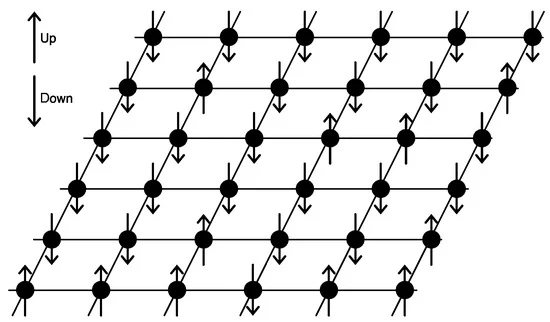
\includegraphics[width=3cm]{ising}}

\pause

\begin{block}{\QMA-hard and \BQP-hard Problems}
\begin{itemize}
\item Finding the ground state / energy
\item Computing the temperature of a system
\item Quantum many-body physics
\end{itemize}
\end{block}

\end{refframe}


\begin{refframe}{Translating Back to Physics}

\centering

\cols{
\col{.5\textwidth}{
{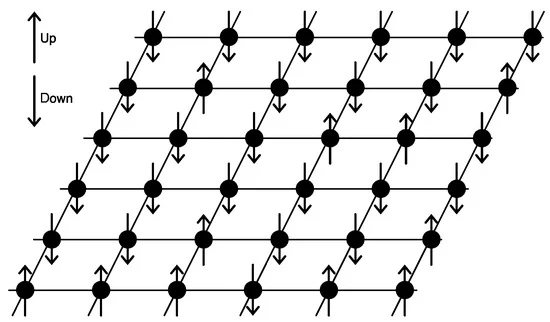
\includegraphics[width=3cm]{ising}}
}
\col{.5\textwidth}{
Physicists use {tensor networks} (e.g. \textbf{MPS}) and restricted Boltzmann Machines (\textbf{RBM}) to analyze these problems\\ (\alert{in very similar ways to our use of DDs!})
}
}

\onslide<2->{
As a first step to unifying these approaches, we give a first ``knowledge compilation map'' for quantum information~\cite{vinkhuijzen2024a}:
}


\begin{columns}<3->
\begin{column}{.45\textwidth}	
\centering
~~~~~~~~\begin{tikzpicture}\footnotesize
  \tikzset{venn circle/.style={circle,minimum width=2cm,fill=####1,opacity=0.6}}
  \node [venn circle=white,minimum width=4cm,draw] (A) at (0,0.3) {};
  \node  at (0,1.95) 			{State space};

  \node [venn circle = Red!40!white, ellipse,minimum height=2.2cm, minimum width=3.6cm] (L) at (0,0.3) {};
  \node  at (0,1.2) 		{poly-\alert{\limdd}};
  
  \node [venn circle = blue!70!white,text width=1.3cm,align=center,rotate=79,ellipse,minimum height=1.8cm, minimum width=2.5cm] (B) at (-.6,-.2) {};
  \node[text width=1.3cm,align=center]  at (-.7,-1.) {poly-MPS};


  \node [venn circle = green!70!white,text width=1.3cm,align=center,rotate=119,ellipse,minimum height=1.8cm, minimum width=2.5cm] (B) at (.6,-.2) {};
  \node[text width=1.3cm,align=center]  at (.9,-1.) {poly-RBM};


  \node [venn circle = Blue!100!white,text width=1cm,align=center, minimum width=1.cm,text opacity=1] (B) at (-.5,.3) 	{\textcolor{white}{poly-QMDD}};						

  \node [venn circle = OliveGreen!100!white,text width=1cm,align=center, minimum width=1.cm,text opacity=1] (C) at (.5,.3) {\textcolor{white}{Stabilizer states}};

\end{tikzpicture}
	\end{column}
	\begin{column}{.65\textwidth}
	\pause
\setlength{\tabcolsep}{2pt}
\def\arraystretch{1.1}
\footnotesize
\begin{tabular}{|l@{\hspace{10pt}}|| *{5}{c|}| *{20}{c|}}
%\footnotesize
\hline
 & \multicolumn{5}{c||}{Queries} & \multicolumn{7}{c|}{Manipulation operations} \\
	& \rot{\samp} & \rot{\pro} & \rot{\eq}  & \rot{\inprod} & \multicolumn{1}{R{90}{0em}||}{\fid}
	& \rot{\addi} & \rot\had & \rot{\xyz} & \rot\cz & \rot{\swap} & \rot{\loc} & \rot{\T-gate} \\
\hline
%Vector& \Yar & \Yes & \Yes & \Yes & \Yes & \Yes & \Yes & \Yes & \Yes & \Yes & \Yes & \Yes \\
%\hline
%		| Sampl	| Prob 	| Eq	|Inprod	| Fid
MTBDD   	& \Yar	& \Yes	& \Yes	& \Yes & \Yes
%		| Add	| H		| XYZ	| CX	| Swap	| Local	| T
		& \Yes	& \Yes 	& \Yes	& \Yes	& \Yes	& \Yes	& \Yes \\
\hline
QMDD
		& \Yar	& \Yes	& \Yes	& \Yes & \Yes
		& \No	& \No 	& \Yes	& \Yes	& \No	& \No	& \Yes \\
\hline 
%QMDD  & \Yes & \Yes & \Yes & \No & \Yes & \No & ?? & ??  & ?? & \No & ?? & ??   \\
%\hline    
{\limdd} 	& \Yar	& \Yes	& \Yes	& \Cond & \Cond
		& \No	& \No	& \Yes	& \Yes	& \No	& \No	& \Yes  \\
\hline 
%TN    & \Cond? & \Cond? & \Cond? & \Cond? & ?? & \Yes? & \Yes? & \Yes? & \Yes? & \Yes? & \Yes? \\ \hline
\alert{MPS}   & \Yar & \Yes & \Yes & \Yes & \Yes & \Yes 
	  & \Yes & \Yes & \Yes & \Yes & \Yes & \Yes  \\
\hline 
\alert{RBM}   & \Yar    & ? & ? & \Cond & \Cond & ? & ? & \Yes & \Yes & \Yes & ? & \Yes \\
\hline 
%\multicolumn{13}{c}{Low priority} \\
%\hline 
%ZX    & ?? & ?? & ?? & ?? & ?? & ?? & ?? & ?? & ?? & ?? & ?? & ?? \\
%\hline 
%SLDD$_+$  & \Yes? & \Yes? & \Yes? & \Yes? & \Yes? & \No! & \No? & \Yes? & \No! & \No! & \No? & \Yes! \\
%\hline 
\end{tabular}

\centering
\Yes = tractable\\
\No = intractable\\
\Cond = conditionally intractable
\end{column}
\end{columns}


\end{refframe}


\begin{refsection}
\begin{frame}{Takeaways and Thank Yous}

\vspace{-1em}

\begin{itemize}
	\item Classical automated reasoning tools are unreasonably effective for quantum
	\item Progress in quantum computing is progress in tackling nature's hardest problems
\end{itemize}


\vspace{2em}

\pause

%\includegraphics[height=2cm]{graphics/thanos.jpg}
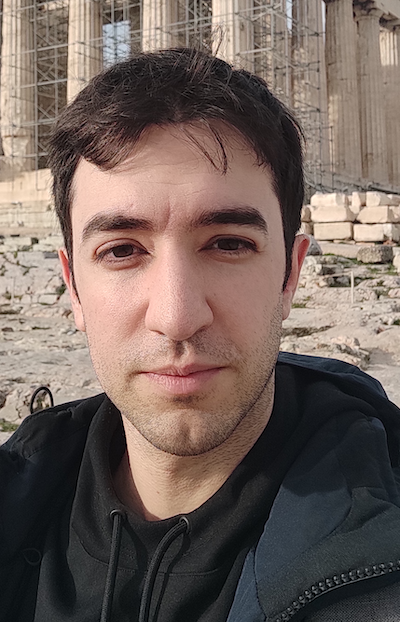
\includegraphics[height=2cm]{graphics/dimitrios}
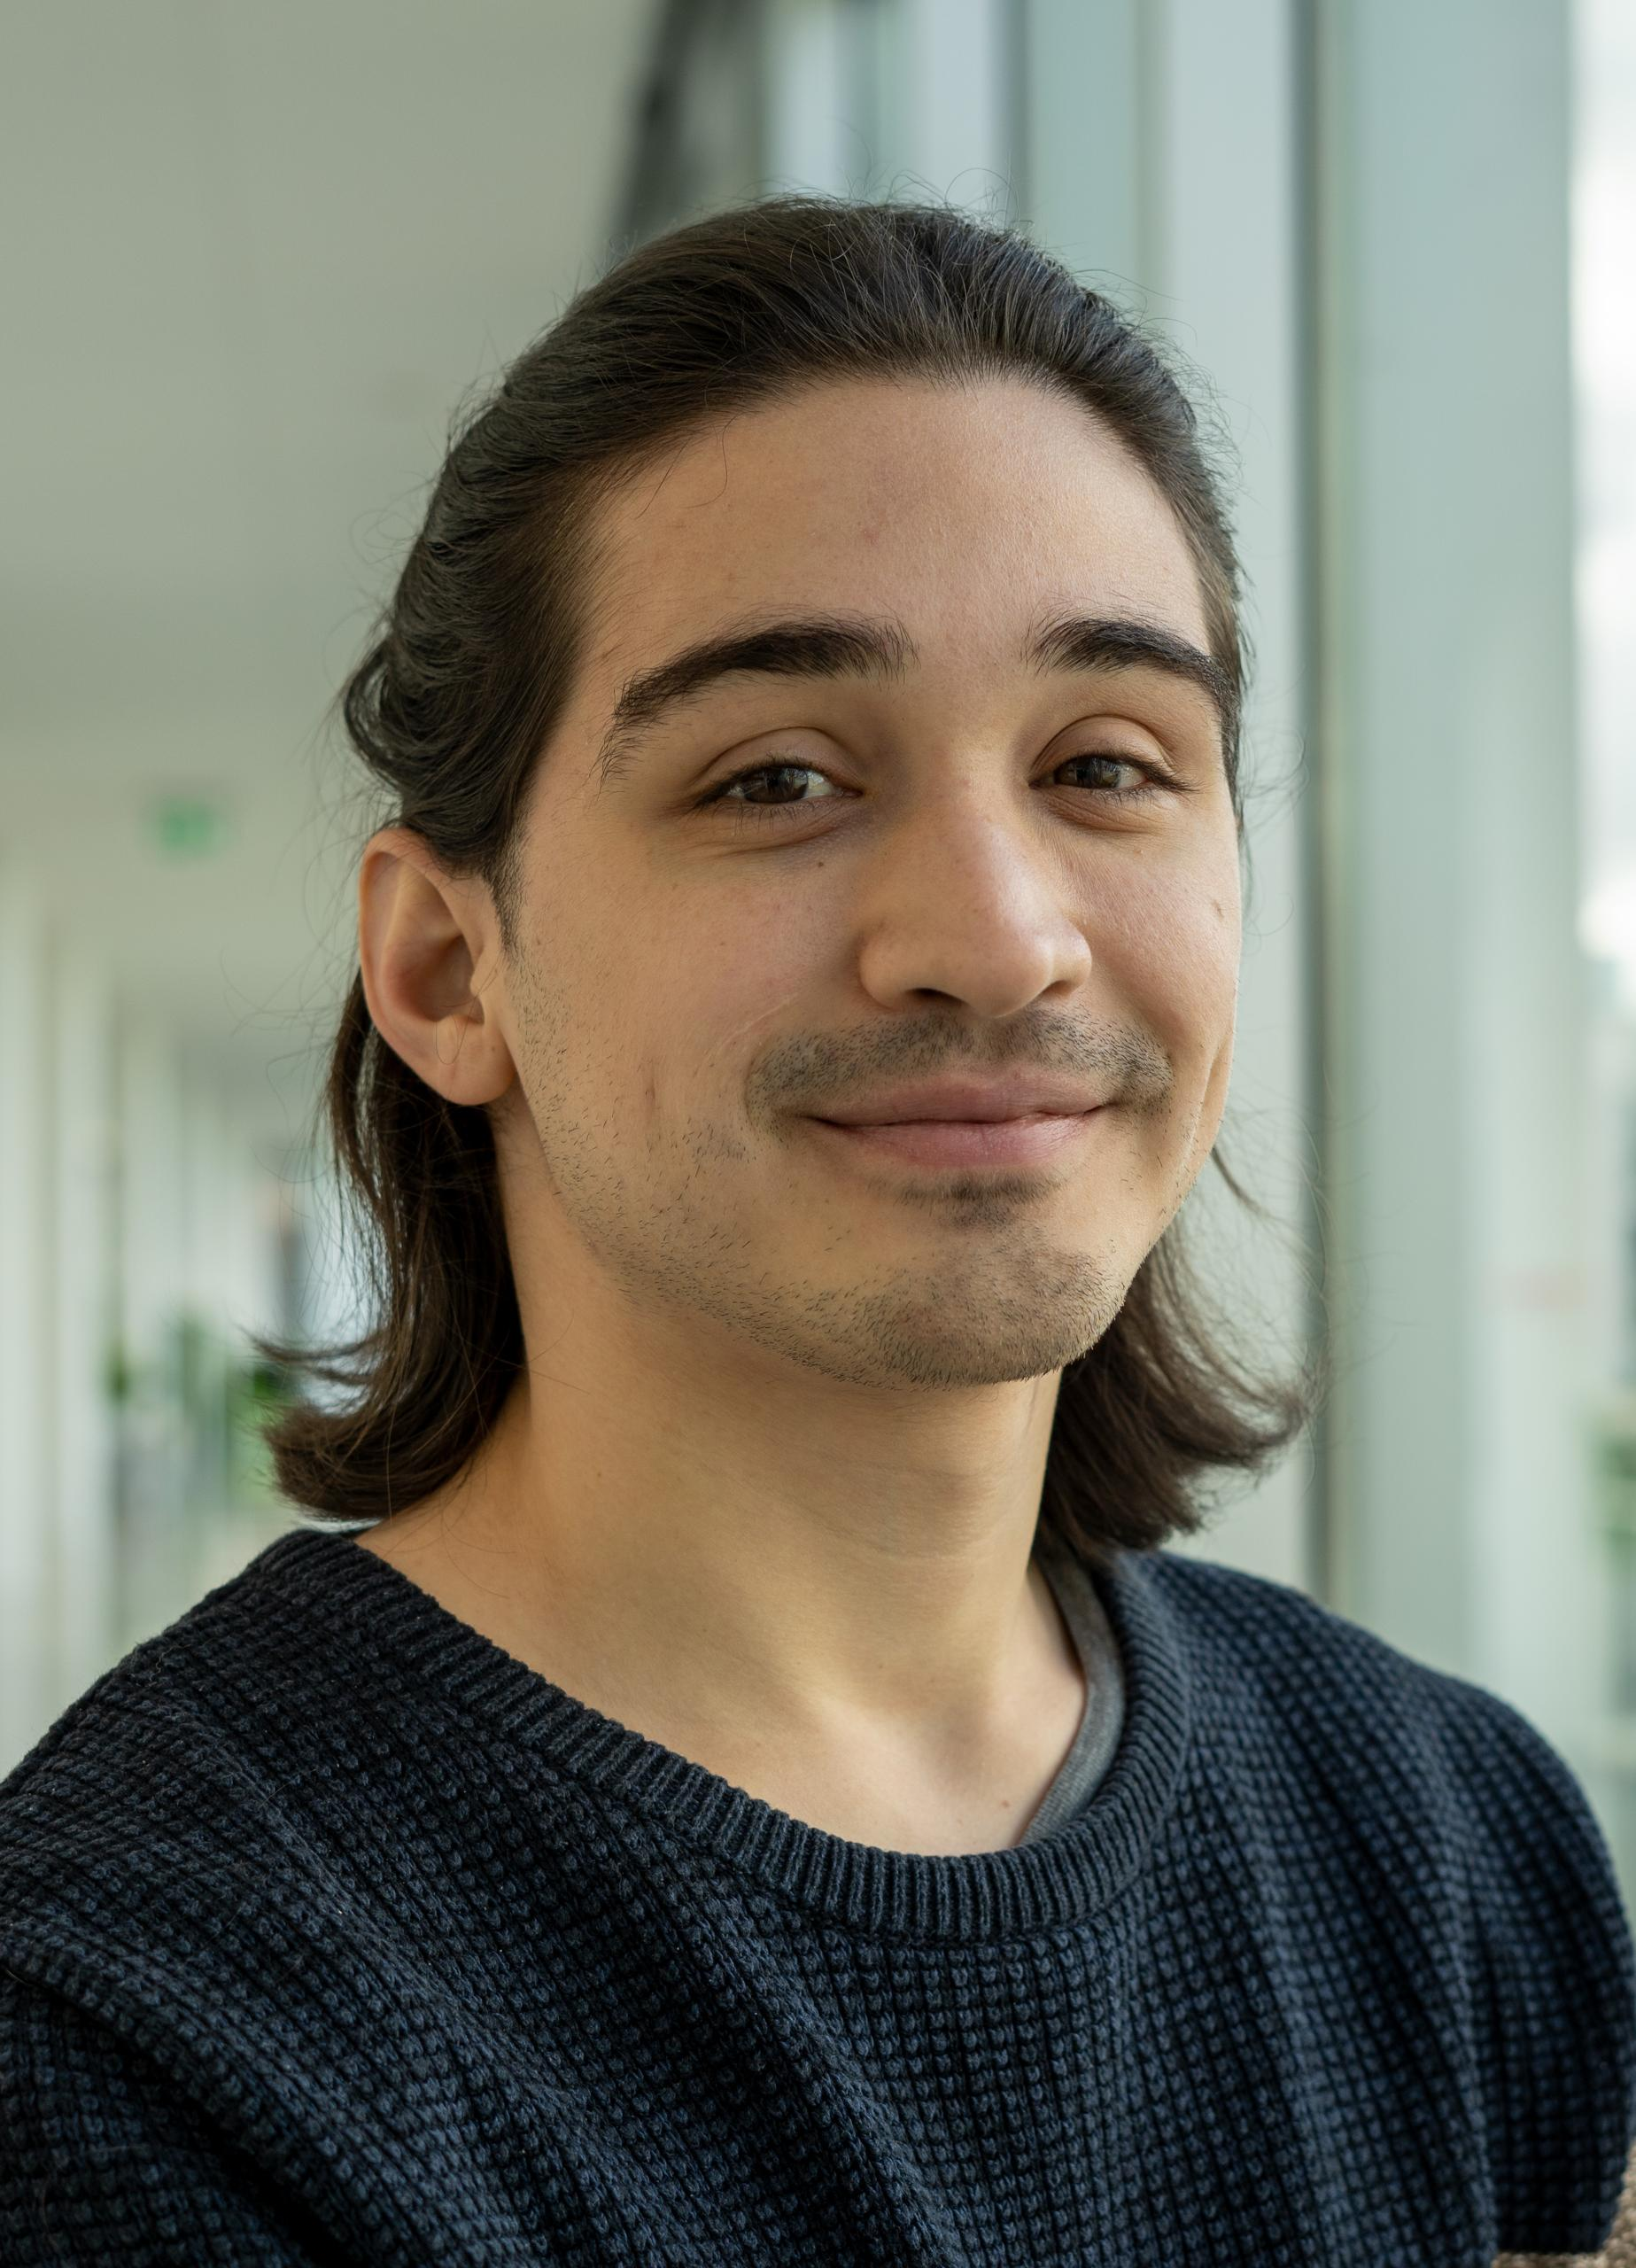
\includegraphics[height=2cm]{graphics/villoria_alejandro.jpg}
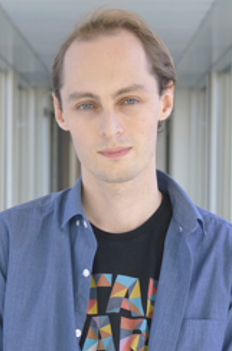
\includegraphics[height=2cm]{graphics/brand.png}
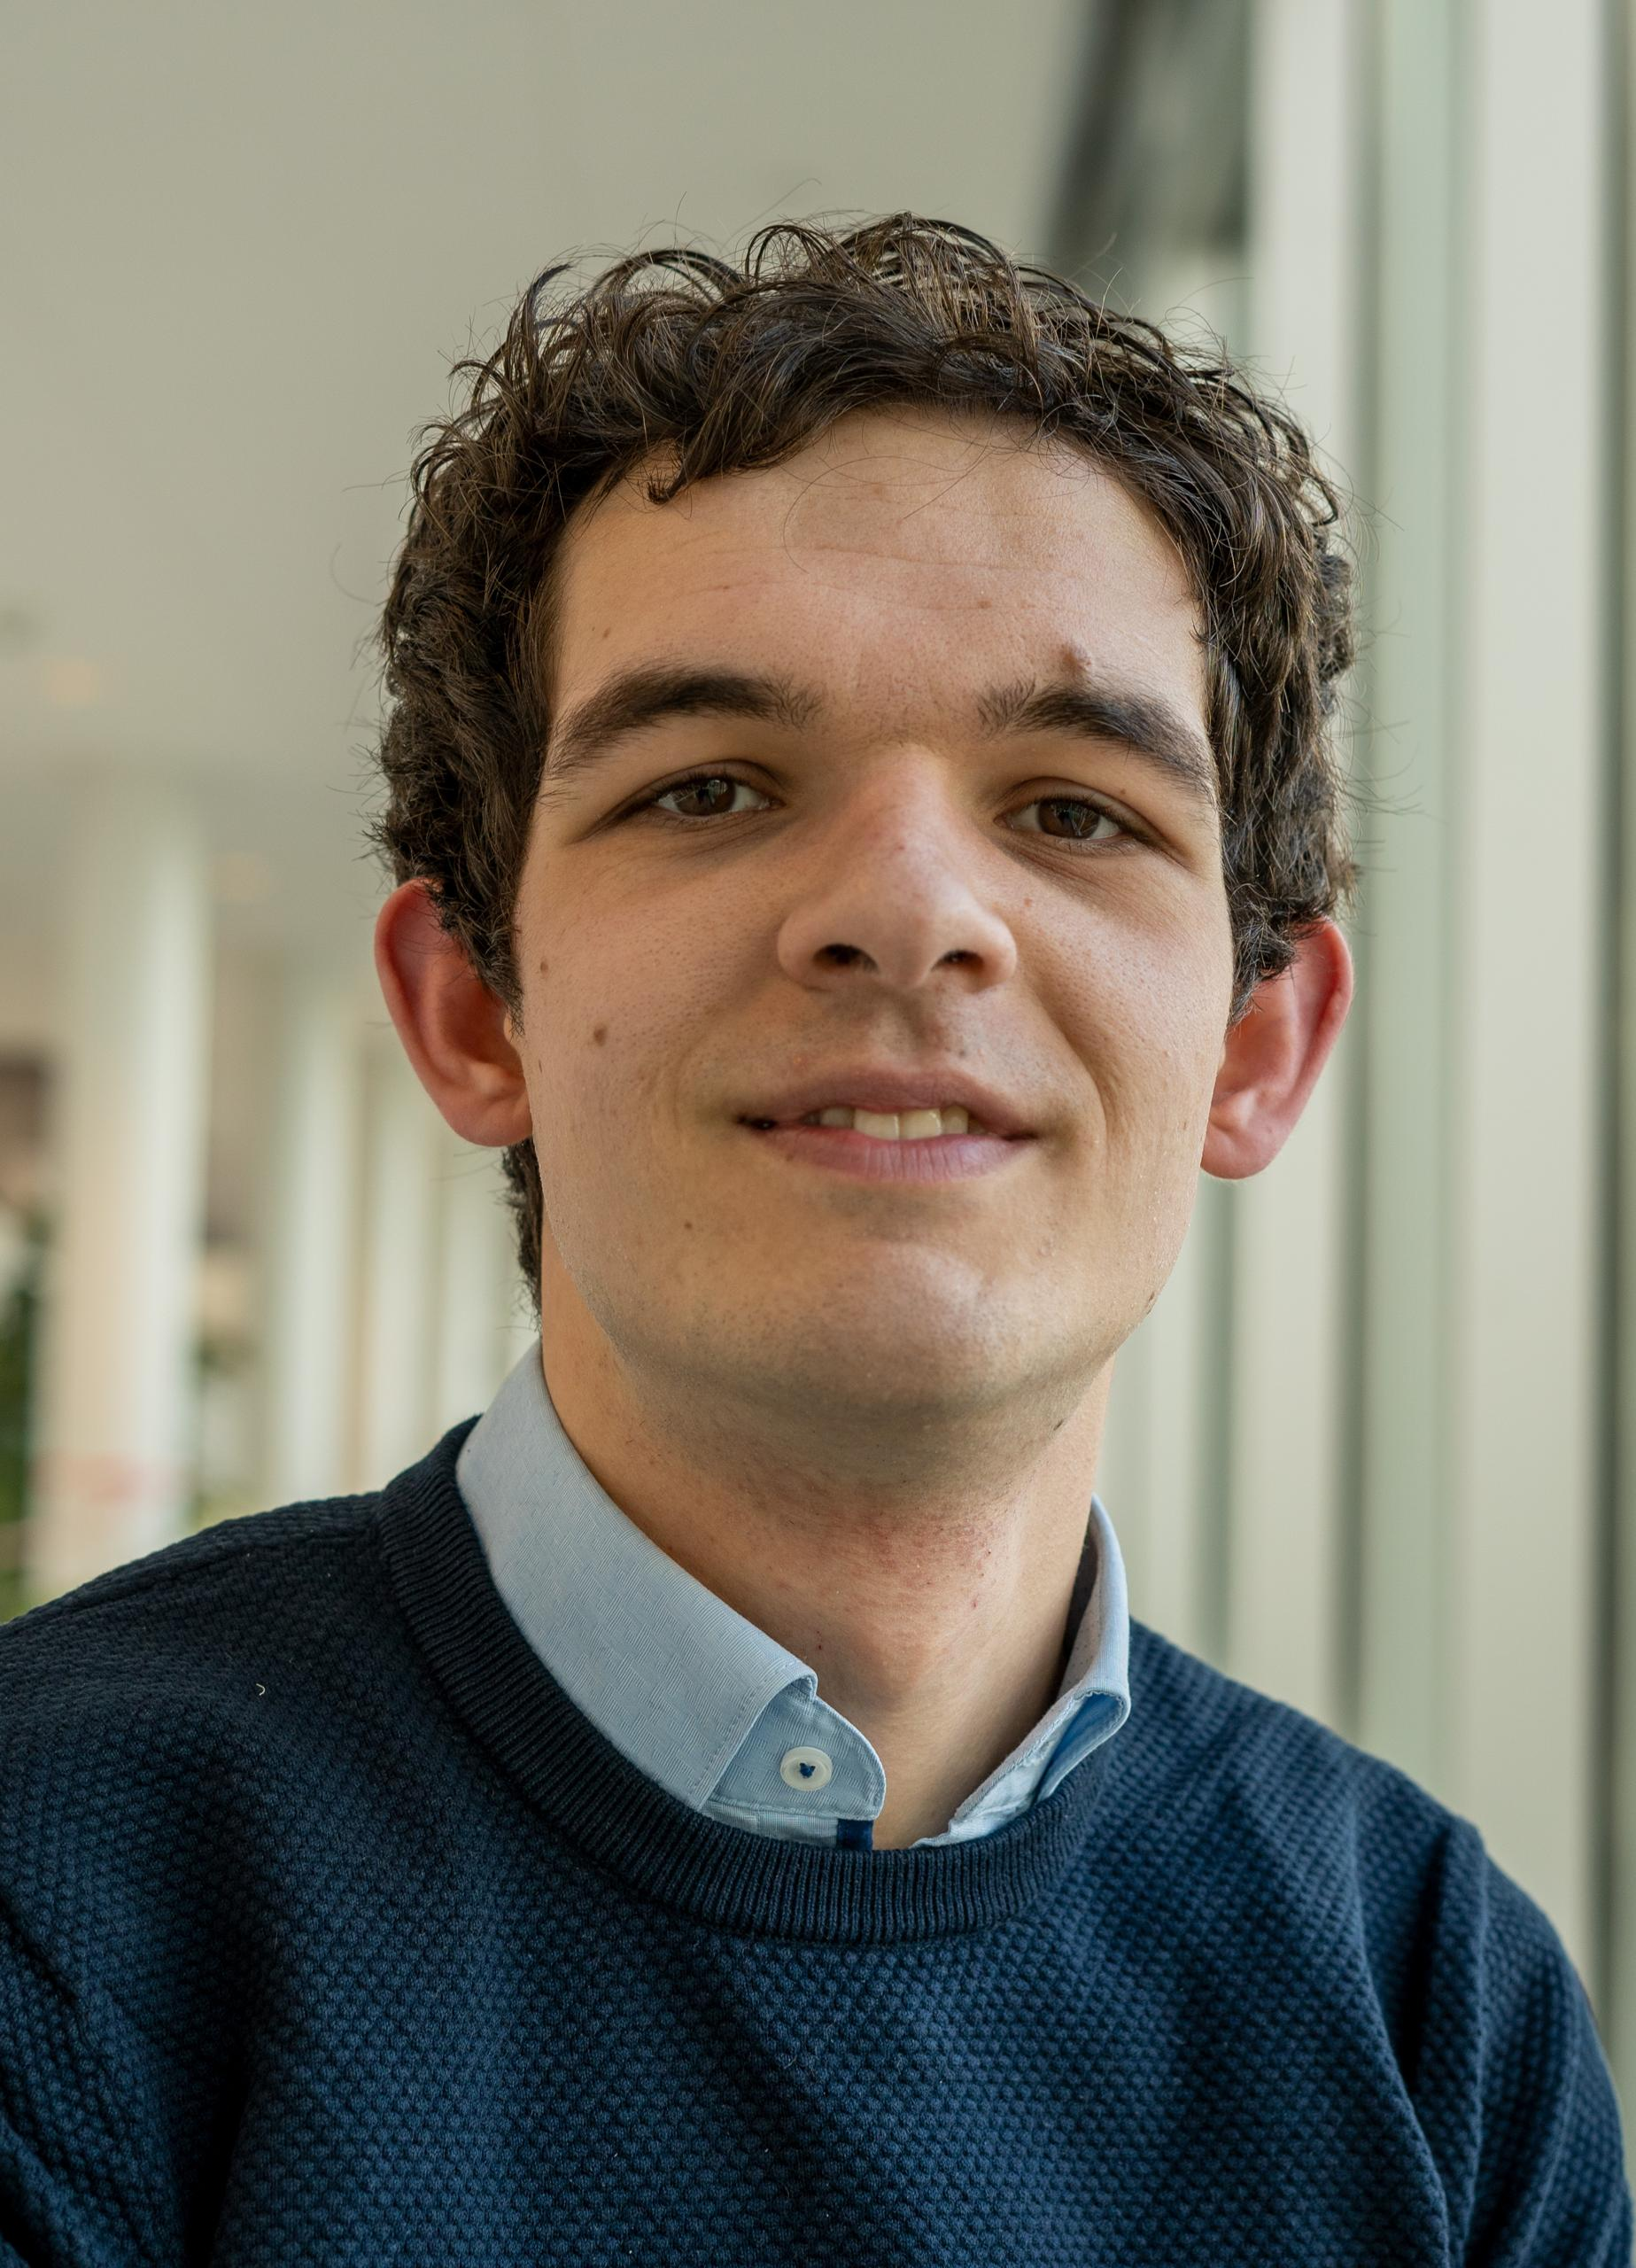
\includegraphics[height=2cm]{graphics/quist_arend-jan.jpg}
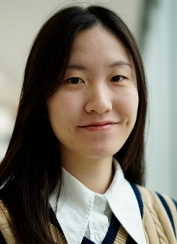
\includegraphics[height=2cm]{graphics/mei.png}
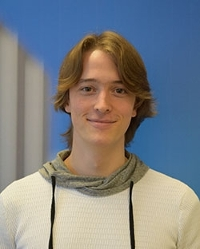
\includegraphics[height=2cm]{graphics/lieuwe.jpeg}
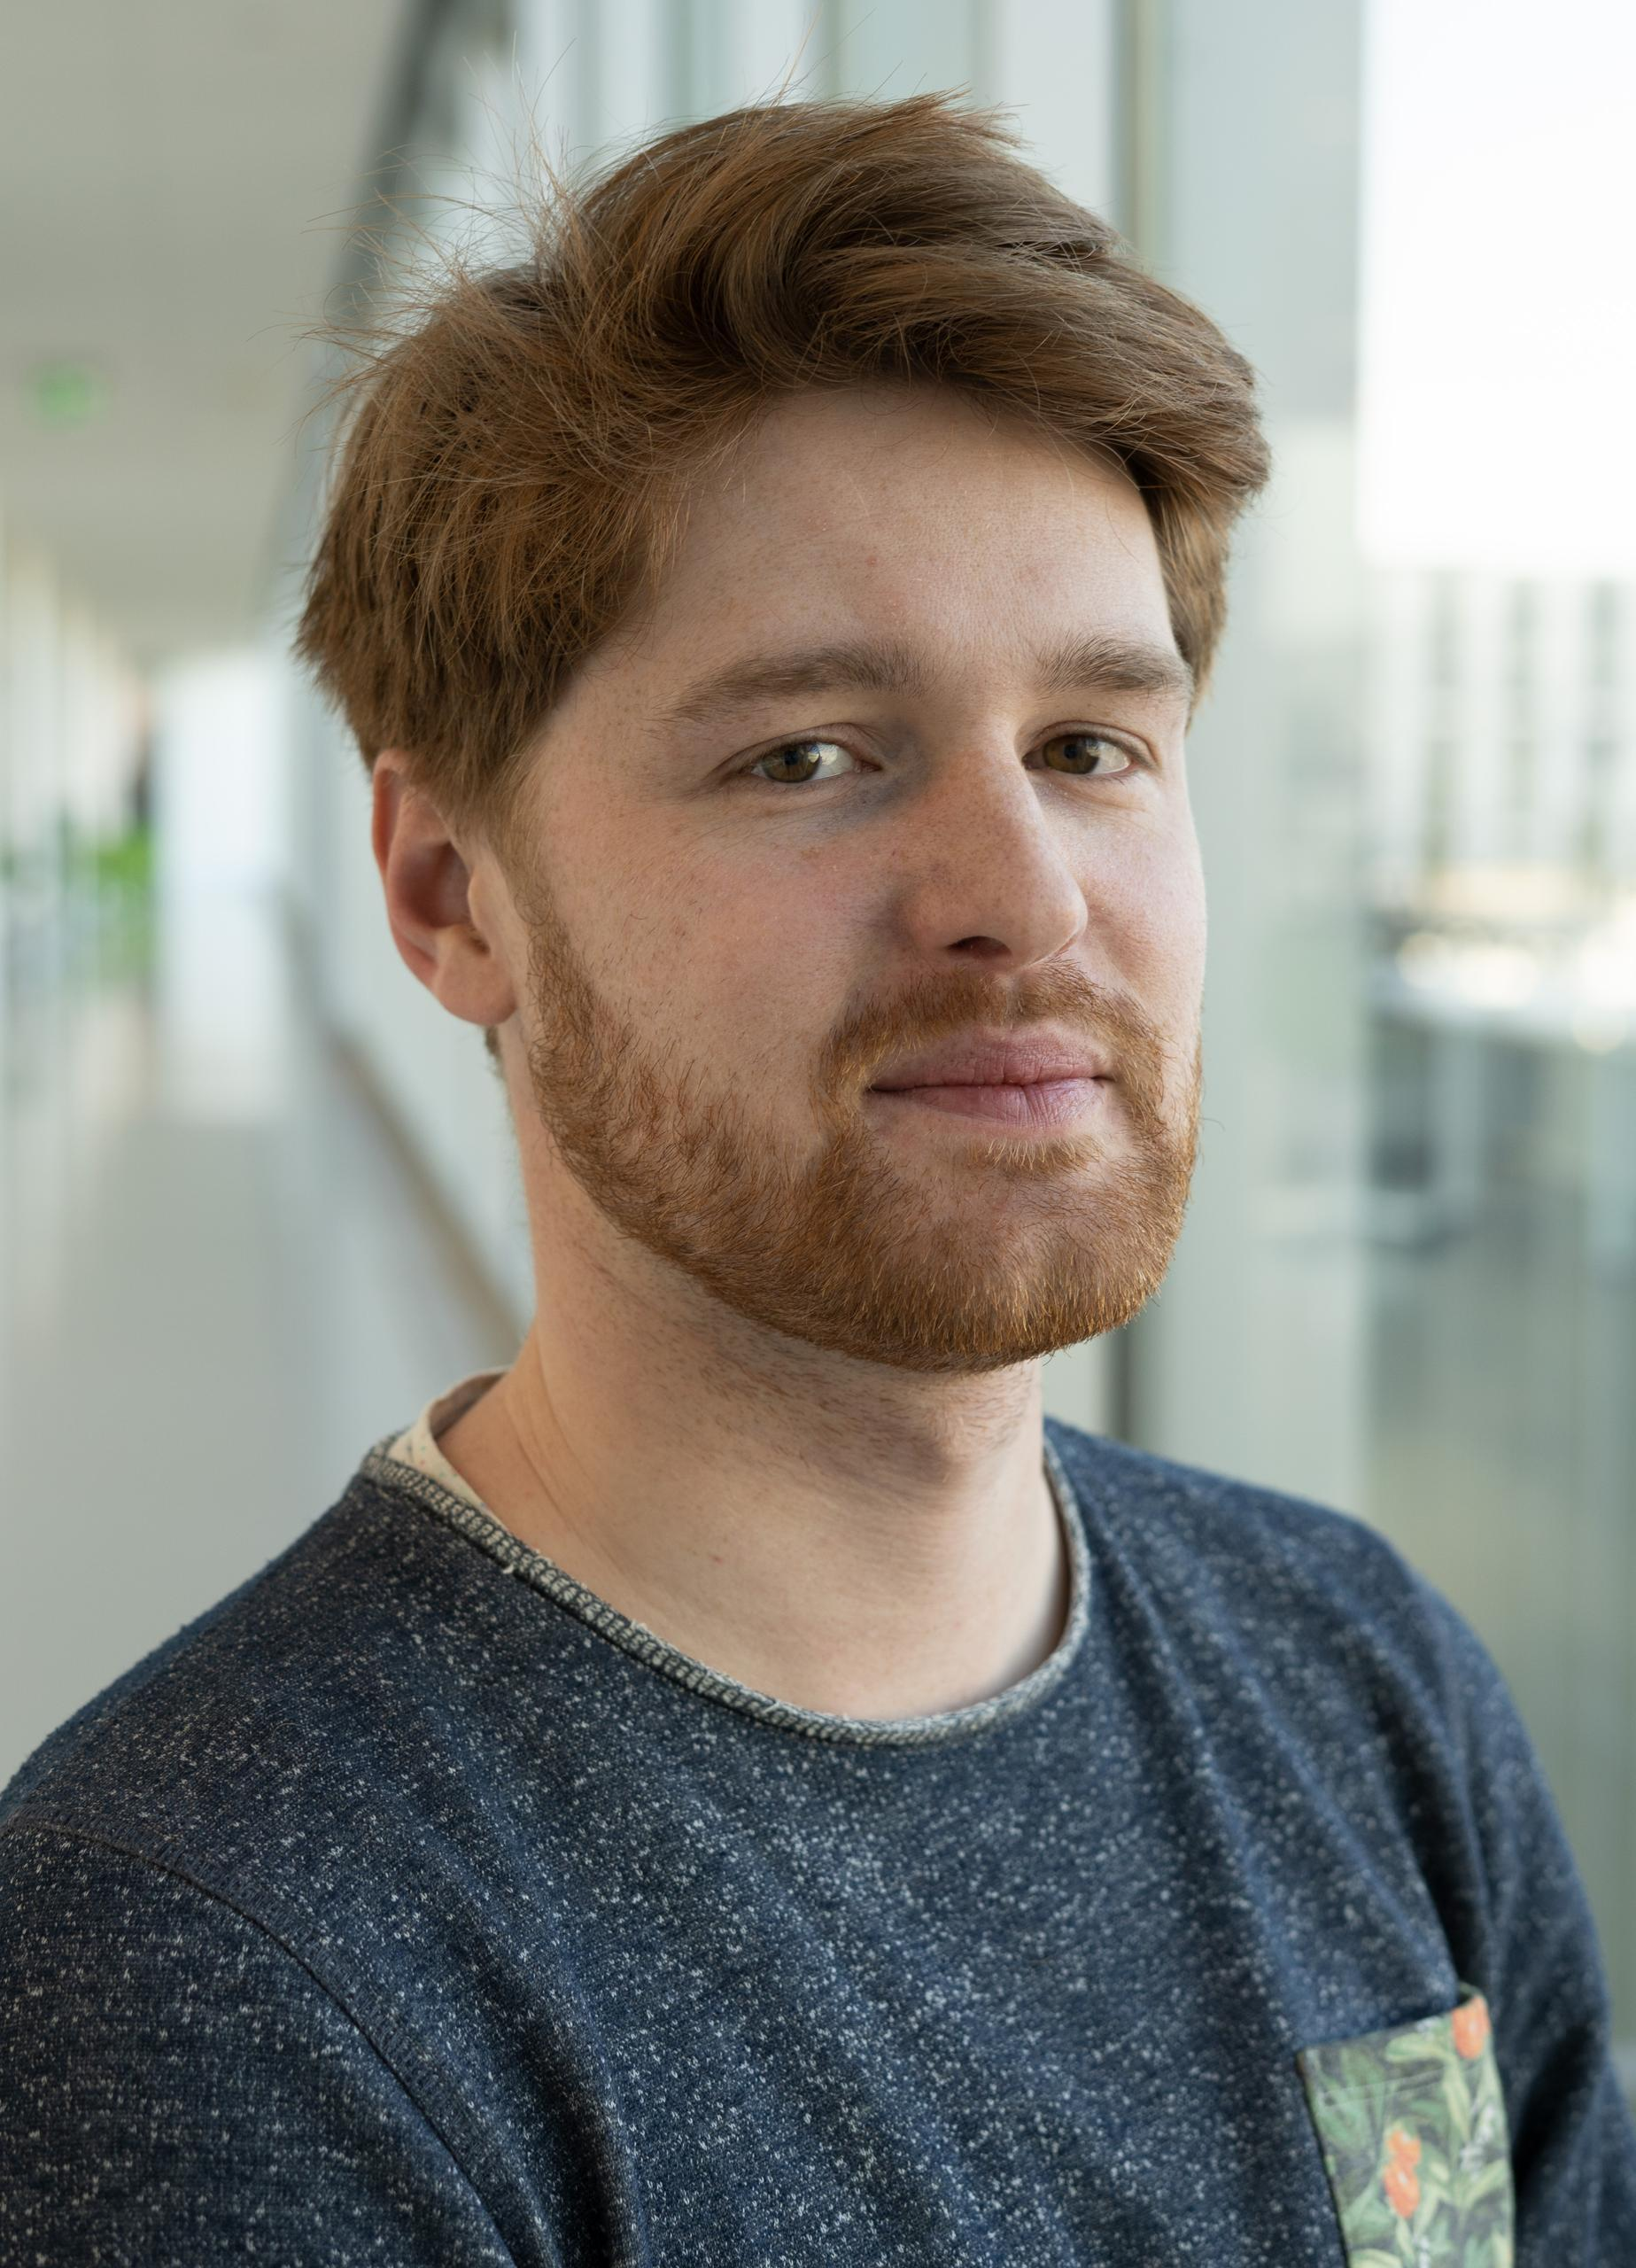
\includegraphics[height=2cm]{graphics/coopmans_tim}
%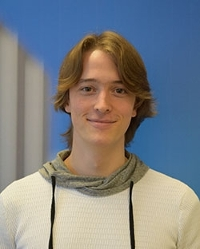
\includegraphics[width=2cm]{graphics/lieuwe}

\footnotesize
Dimitrios Thanos~~~~~~~~~~~~~~
Sebastiaan Brand~~~~~~~~~~~~~~~~~~~~~~ 
Jingyi Mei~~~~~~~~~~~~~~~~~~~~~~~~~~~
Tim Coopmans

\vspace{-2ex}
~~~~~~~~~~~~~~~~~
Alejandro Villoria~~~~~~~~~~~~~~~~~
Arend-Jan Quist~~~~~~~~~~~~~~~~~~~
Lieuwe Vinkhuijzen


\vspace{-1em}

\phantom{\cite{limdd,vinkhuijzen2024a,mei2024simulating,mei2024eq,ours}}


%\vfill
%\centering
%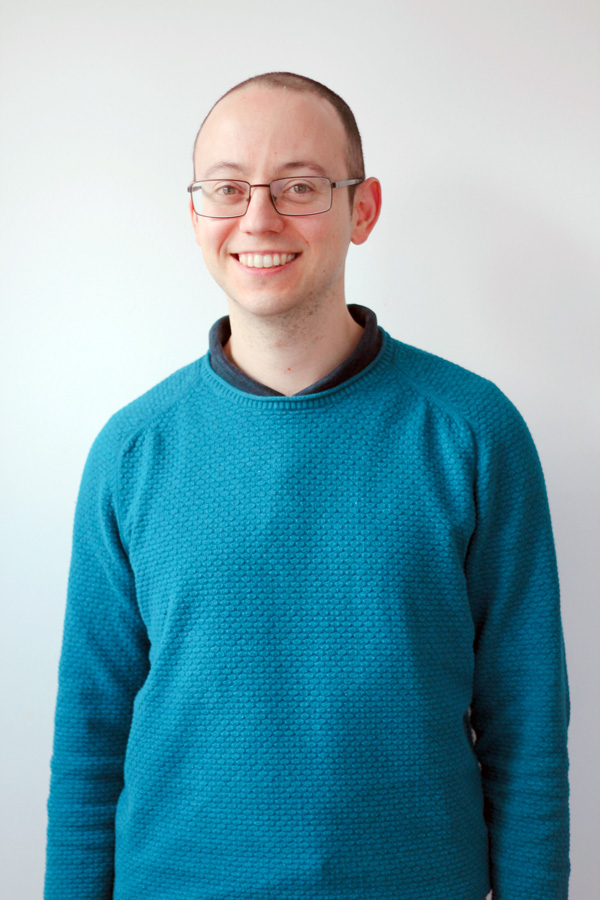
\includegraphics[height=2cm]{graphics/elkouss-david-20211227-torso_0}
%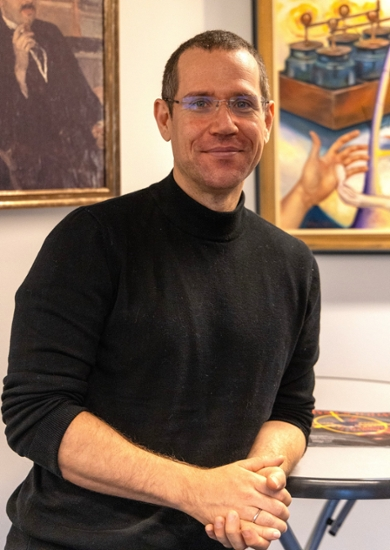
\includegraphics[height=2cm]{graphics/vedran-jobs}
%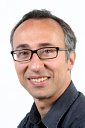
\includegraphics[height=2cm]{graphics/bonsangue}
%
%~~David Elkouss (Okinawa, Delft) ~~~
%Marcello Bonsangue (Leiden)

%\vspace{-2ex}
%Vedran Dunjko (Leiden)


\printbibliography[section=\therefsection]
\end{frame}
\end{refsection}




